The floor on which the user can build is divided into squares of $1 \times 1$ unit, in which the user can build conveyor belts and scanners. We will call such objects \textit{blocks}. The blocks also have size $1 \times 1$, and the user can only put a block exactly inside a square. There are several blocks for conveyor belts, for example a block with a horizontal conveyor belt, a block with a sloped conveyor belt and a block with a bended conveyor belt. The user does not explicitly have to choose between those conveyor belt blocks, but this is chosen automatically most of the time. The user is able to change the orientation of blocks manually however (but only in steps of $90\,^\circ$), thus changing the type of block and possibly that of the neighbouring blocks too.

\begin{figure}
  \begin{center}
    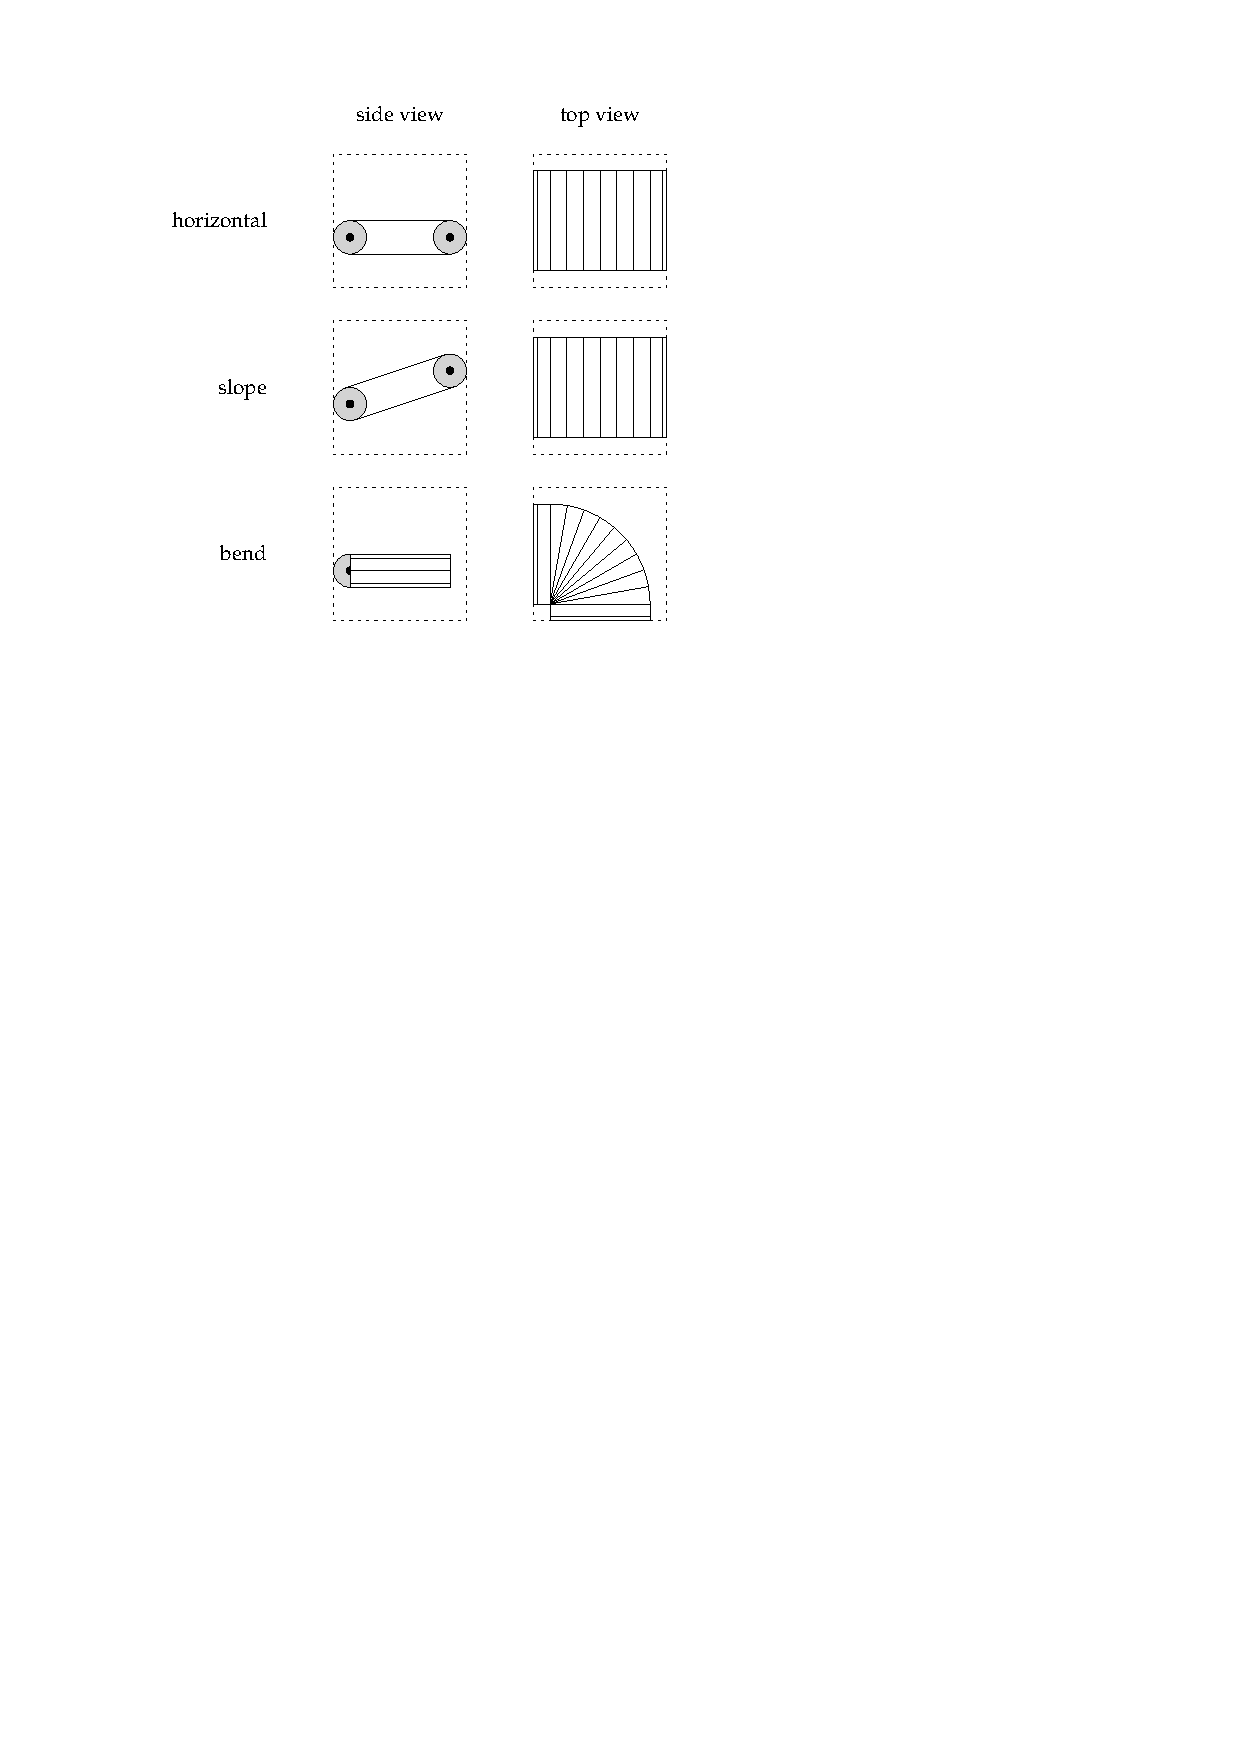
\includegraphics{blocks-sketch}
    \caption{Different types of conveyor belt blocks.}
    \label{fig:block-types}
  \end{center}
\end{figure}

The user can also stack blocks. Every block has a height of $1/2$ unit \textbf{(dat is niet waar, stijgende blokken hebben een hoogte van $1$ unit)}.

If the user places two blocks with the same orientation adjacent to each other, they will be drawn as one long conveyor belt. This also happens when a horizontal block is joined with a sloped block. See Figure~\ref{fig:blocks}.

\begin{figure}
  \begin{center}
    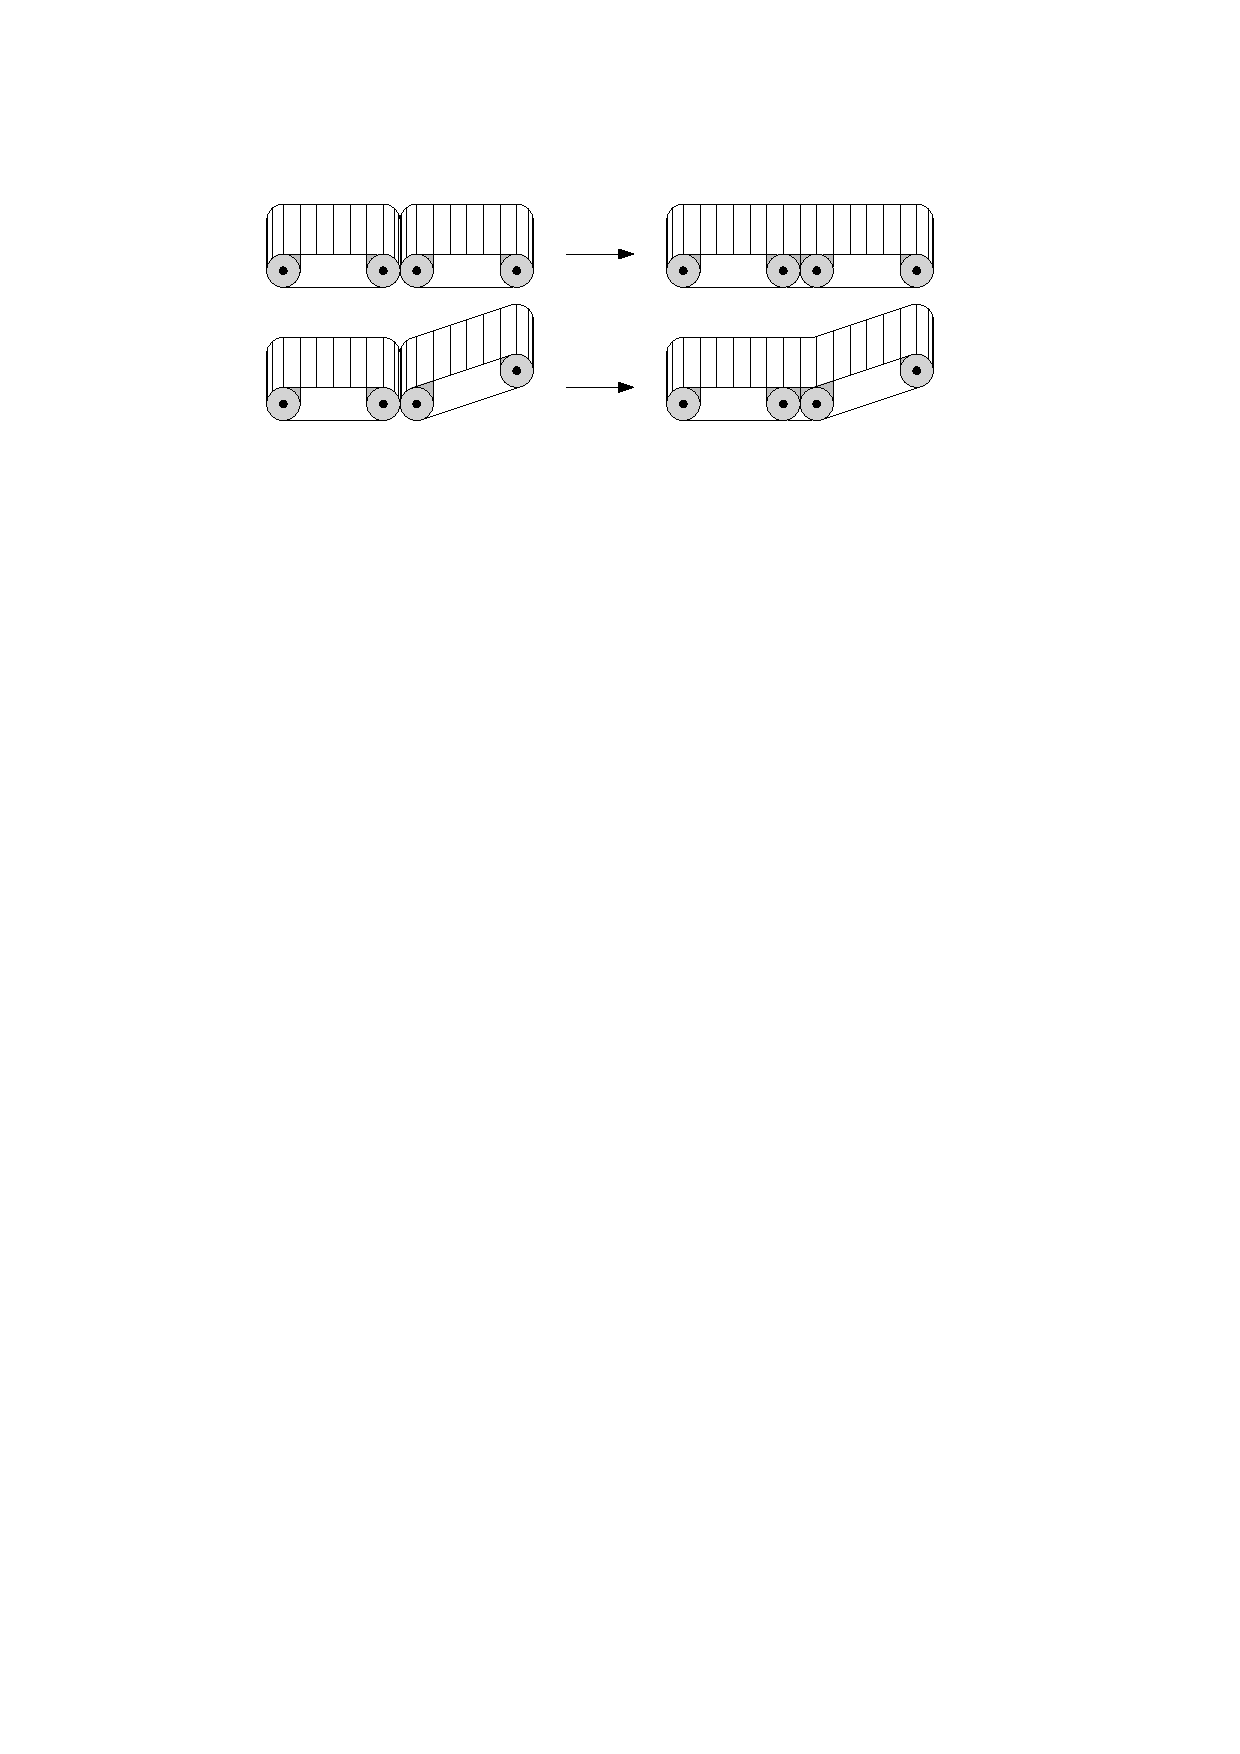
\includegraphics{blocks}
    \caption{Adjacent blocks are drawn as one large conveyor belt.}
    \label{fig:blocks}
  \end{center}
\end{figure}

Next to conveyor belt blocks, there are also \textit{scanners}. These blocks can send a piece of luggage to one of its two outputs, depending on its type. We think that it is fun in a game form of this program to make the user sort the luggage that comes in using these scanners. The type of luggage can be indicated by colours, as can the scanners. This is also shown in the mock-up in Figure~\ref{fig:mockup}. It may also be useful when this program would be used to design luggage handling systems for airports, because there luggage has to go to a specific exit (for a specific flight for example).